\documentclass{standalone}
\usepackage{tikz}
\begin{document}
	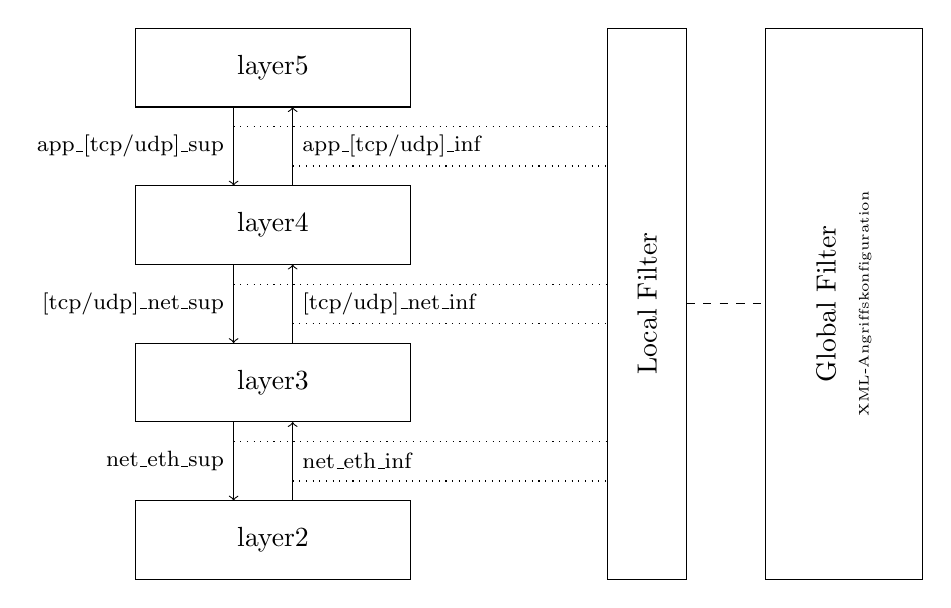
\begin{tikzpicture}	
		\draw (0, 0) rectangle (3.5,-1) node[pos=.5] {\gls{layer5}};
		\draw (0, -2) rectangle (3.5,-3) node[pos=.5] {\gls{layer4}};
		\draw (0, -4) rectangle (3.5,-5) node[pos=.5] {\gls{layer3}};
		\draw (0, -6) rectangle (3.5,-7) node[pos=.5] {\gls{layer2}};
		
		\draw[draw=black] (6,0) rectangle node[pos=.5,rotate=90] {Local Filter} (7, -7);
		
		\draw[draw=black] (8,0) rectangle node[pos=.5,rotate=90, align=center] {Global Filter \\ \tiny XML-Angriffskonfiguration} (10, -7);
		\draw[dashed] (7, -3.5) -- (8,-3.5);
		
		\path[draw, ->] (1.25, -1) -- node[left, midway] (1) {\footnotesize app\textunderscore[tcp/udp]\textunderscore{}sup} (1.25,-2);
		\path[draw, <-] (2, -1) -- node[right, midway] (2) {\footnotesize app\textunderscore[tcp/udp]\textunderscore{}inf} (2,-2);
		
		\draw[dotted] (1.25, -1.25) -- (6,-1.25);
		\draw[dotted] (2, -1.75) -- (6,-1.75);
		
		\path[draw, ->] (1.25, -3) -- node[left, midway] (3) {\footnotesize [tcp/udp]\textunderscore{}net\textunderscore{}sup} (1.25,-4);
		\path[draw, <-] (2, -3) -- node[right, midway] (4) {\footnotesize [tcp/udp]\textunderscore{}net\textunderscore{}inf} (2,-4);
		
		\draw[dotted] (1.25, -3.25) -- (6,-3.25);
		\draw[dotted] (2, -3.75) -- (6,-3.75);
		
		\path[draw, ->] (1.25, -5) -- node[left, midway] (3) {\footnotesize net\textunderscore{}eth\textunderscore{}sup} (1.25,-6);
		\path[draw, <-] (2, -5) -- node[right, midway] (4) {\footnotesize net\textunderscore{}eth\textunderscore{}inf} (2,-6);
		
		\draw[dotted] (1.25, -5.25) -- (6,-5.25);
		\draw[dotted] (2, -5.75) -- (6,-5.75);
\end{tikzpicture}
\end{document}